\documentclass[12pt, twoside]{book}
%\documentclass[12pt, oneside]{book}  % jednostranna tlac

%spravne nastavenie okrajov
\usepackage[a4paper,top=2.5cm,bottom=2.5cm,left=3.5cm,right=2cm]{geometry}
%zapnutie fontov pre UTF8 kodovanie
\usepackage[utf8]{inputenc}
\usepackage[T1]{fontenc}

%zapnutie slovenskeho delenia slov
%a automatickych nadpisov ako Obsah, Obrázok a pod. v slovencine
\usepackage[slovak]{babel} % vypnite pre prace v anglictine!

%nastavenie riadkovania podla smernice
\linespread{1.25} % hodnota 1.25 by mala zodpovedat 1.5 riadkovaniu

% balicek na vkladanie zdrojoveho kodu
\usepackage{listings}

% nastavenia balicka listings
\renewcommand{\lstlistingname}{Úryvok}
\lstset{extendedchars=true, basicstyle=\footnotesize, frame=lines, tabsize=4,
    commentstyle=\color{olive}\textit, keywordstyle=[1]\color{blue},
    literate=
    {á}{{\'a}}1 {ä}{{\"a}}1 {č}{{\v{c}}}1 {ď}{{\v{d}}}1 {é}{{\'e}}1 {í}{{\'i}}1
    {ĺ}{{\'l}}1 {ľ}{{\v{l}}}1 {ň}{{\v{n}}}1 {ó}{{\'o}}1 {ô}{{\^o}}1 {š}{{\v{s}}}1
    {ť}{{\v{t}}}1 {ú}{{\'u}}1 {ý}{{\'y}}1 {ž}{{\v{z}}}1
    {Á}{{\'A}}1 {Č}{{\v{C}}}1 {Ď}{{\v{D}}}1 {É}{{\'E}}1 {Í}{{\'I}}1 {Ĺ}{{\'L}}1 
    {Ľ}{{\v{L}}}1 {Ň}{{\v{N}}}1 {Ó}{{\'O}}1 {Š}{{\v{S}}}1 {Ť}{{\v{T}}}1 {Ú}{{\'U}}1
    {Ý}{{\'Y}}1 {Ž}{{\v{Z}}}1
    {~}{{$\sim$}}1 {-}{{\textendash}}1,
}
\lstdefinelanguage{AVR}{
    keywords={clr, eor, cpi, breq, inc, tst, brne, ldi, sbi, cbi, nop, add, sub, mov, or, dec, ldr, str},
    sensitive=false,
    comment=[l]{;},
}

% balicek na vkladanie obrazkov
\usepackage{graphicx}
\usepackage{subfig}
% balicek pre pouzitie hrubych ciar
\usepackage{boldline}
% balicek pre viacriadkove tabulky
\usepackage{multirow}
% balicek na vkladanie celych pdf dokumentov
\usepackage{pdfpages}
% balicek na vkladanie diagramov
\usepackage{pgfplots}
\pgfplotsset{width=0.6\textwidth,compat=1.9}
% balicek na spravne formatovanie URL
\usepackage{url}
% balicek na hyperlinky v ramci dokumentu
% zrusime farebne ramiky okolo liniek
\usepackage[hidelinks,breaklinks]{hyperref}



% -------------------
% --- Definicia zakladnych pojmov
% --- Vyplnte podla vasho zadania, rok ma byt rok odovzdania
% -------------------
\def\mfrok{2025}
\def\mfnazov{Hardvérové MITM útoky\\na komunikáciu po zberniciach}
\def\mftyp{Diplomová práca}
\def\mfautor{Bc. Dennis Vita}
\def\mfskolitel{RNDr. Richard Ostertág, PhD. }

\def\mfmiesto{Bratislava, \mfrok}

\def\mfodbor{ Informatika}
\def\program{ Informatika }
\def\mfpracovisko{ FMFI.KI - Katedra informatiky }

\begin{document}
\frontmatter
\pagestyle{empty}

% -------------------
% --- Obalka ------
% -------------------
\begin{center}
\sc\large
Univerzita Komenského v Bratislave\\
Fakulta matematiky, fyziky a informatiky

\vfill

{\LARGE\mfnazov}\\
\mftyp
\end{center}

\vfill

{\sc\large 
\noindent \mfrok\\
\mfautor
}

\cleardoublepage
% --- koniec obalky ----


% -------------------
% --- Titulný list
% -------------------
\noindent
\setcounter{page}{1}

\begin{center}
\sc  
\large
Univerzita Komenského v Bratislave\\
Fakulta matematiky, fyziky a informatiky

\vfill

{\LARGE\mfnazov}\\
\mftyp
\end{center}

\vfill

\noindent
\begin{tabular}{ll}
Študijný program: & \program \\
Študijný odbor: & \mfodbor \\
Školiace pracovisko: & \mfpracovisko \\
Školiteľ: & \mfskolitel \\
\end{tabular}

\vfill


\noindent \mfmiesto\\
\mfautor

\cleardoublepage
% --- Koniec titulnej strany


% -------------------
% --- Zadanie z AIS
% -------------------
\newpage 
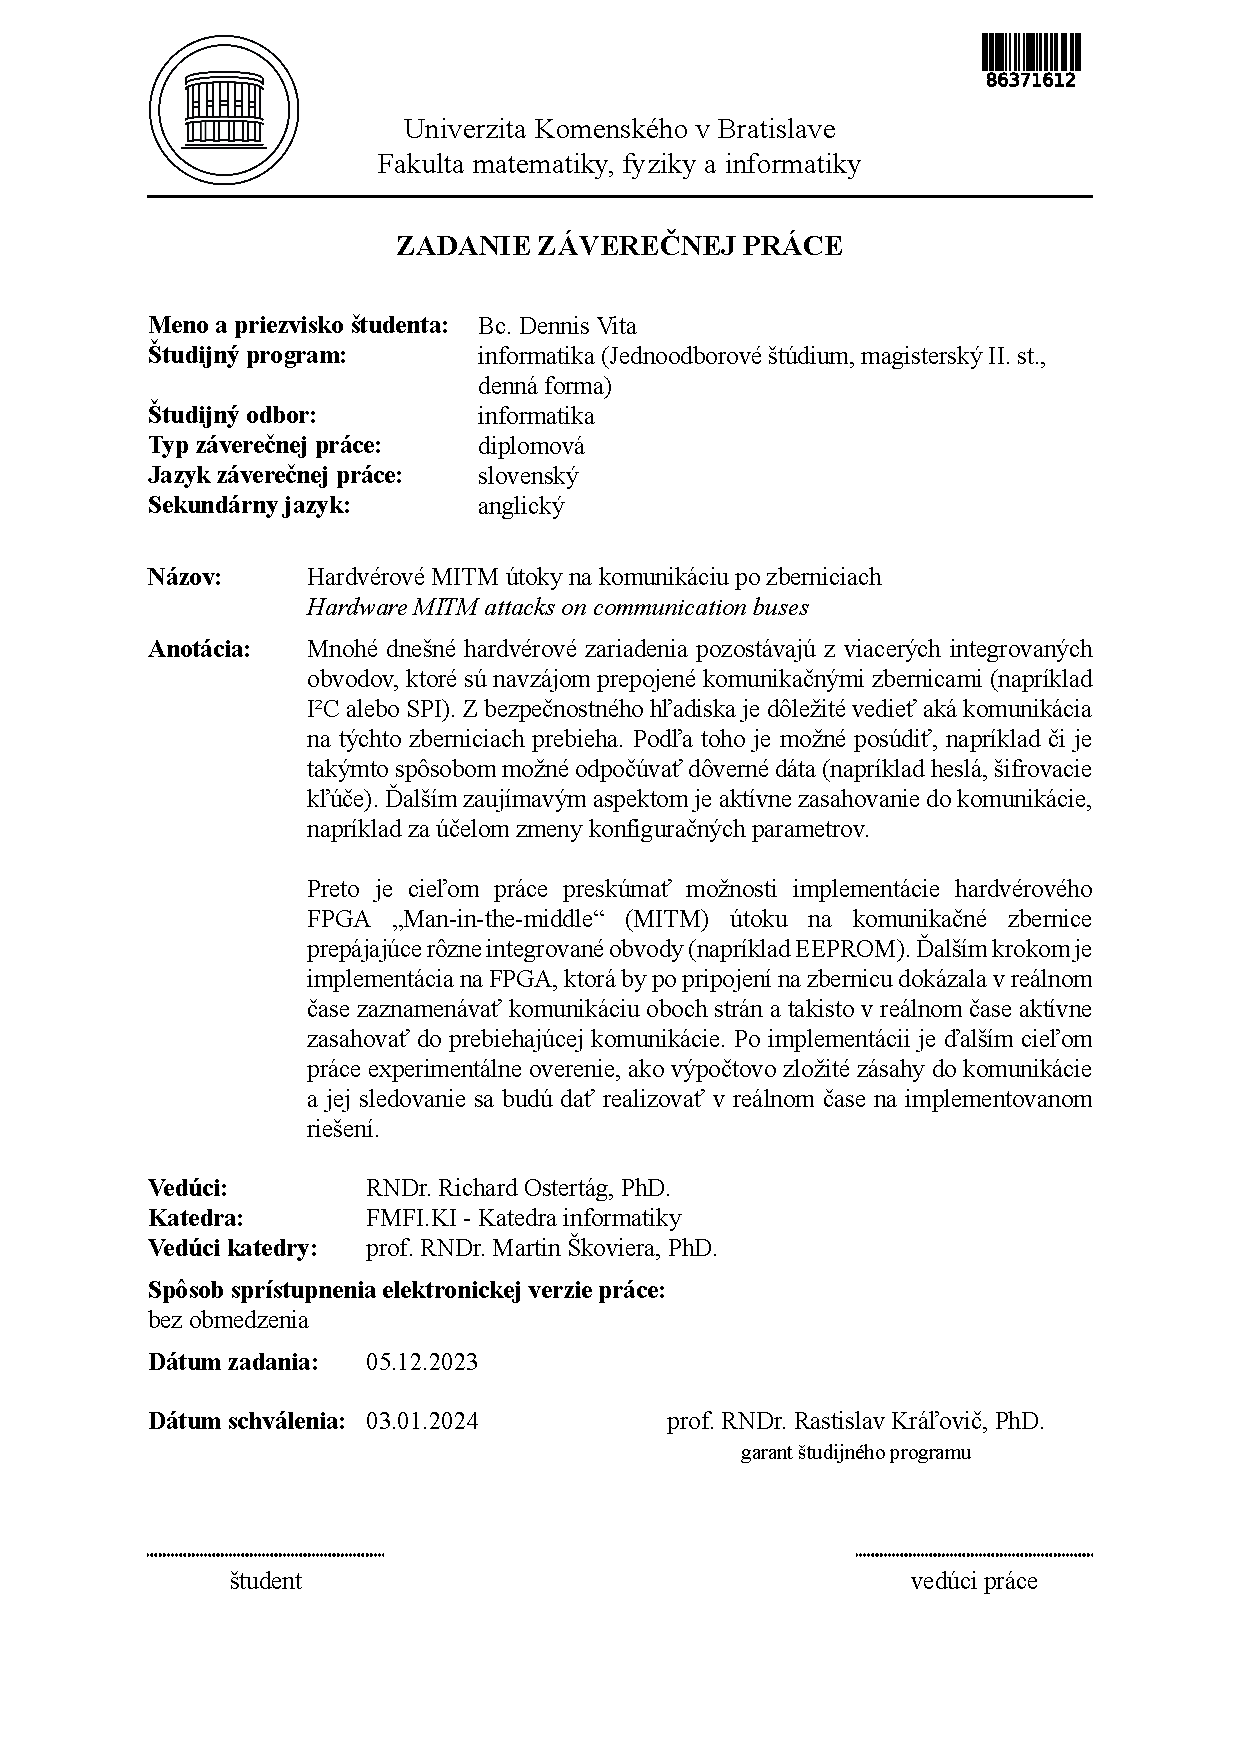
\includepdf{images/zadanie.pdf}

\cleardoublepage
% --- Koniec zadania


% -------------------
%   Poďakovanie - nepovinné
% -------------------
\newpage
\pagestyle{plain}
~

\vfill
{\bf Poďakovanie:} <TO DO> Text poďakovania.
% --- Koniec poďakovania


% -------------------
%   Abstrakt - Slovensky
% -------------------
\newpage 
\section*{Abstrakt}

<TO DO> Abstrakt v slovenskom jazyku.

\paragraph*{Kľúčové slová:} <TO DO>
% --- Koniec Abstrakt - Slovensky


% -------------------
% --- Abstrakt - Anglicky 
% -------------------
\newpage 
\section*{Abstract}

<TO DO> Abstract in the English language.


\paragraph*{Keywords:} <TO DO>
% --- Koniec Abstrakt - Anglicky


% -------------------
% --- Predhovor - v informatike sa zvacsa nepouziva
% -------------------
%\newpage 
%
%\chapter*{Predhovor}
%
%Predhovor je všeobecná informácia o práci, obsahuje hlavnú charakteristiku práce 
%a okolnosti jej vzniku. Autor zdôvodní výber témy, stručne informuje o cieľoch 
%a význame práce, spomenie domáci a zahraničný kontext, komu je práca určená, 
%použité metódy, stav poznania; autor stručne charakterizuje svoj prístup a svoje 
%hľadisko. 
%
% --- Koniec Predhovor


% -------------------
% --- Obsah
% -------------------
\newpage 

\tableofcontents
% ---  Koniec Obsahu


% -------------------
% --- Zoznamy tabuliek, obrázkov - nepovinne
% -------------------
\newpage 

\listoffigures
\listoftables
% ---  Koniec Zoznamov


\mainmatter
\pagestyle{headings}


\input 00-uvod.tex 

\input 01-principy.tex

\input 02-zbernice.tex

\input 03-implementacia.tex

\input 04-priklady.tex

\input 05-zaver.tex


% -------------------
% --- Bibliografia
% -------------------
\newpage	

\backmatter

\thispagestyle{empty}
\clearpage

\bibliographystyle{plain}
\bibliography{literatura} 
%---koniec Referencii


% -------------------
%--- Prilohy---
% -------------------

\input 06-prilohaCD.tex

\end{document}